\documentclass[10pt]{beamer}
\usetheme[progressbar=frametitle]{metropolis}
\usepackage{appendixnumberbeamer}
\usepackage{booktabs}
\usepackage[scale=2]{ccicons}
\usepackage{braket}
\usepackage{pgfplots}
\usepgfplotslibrary{dateplot}
\usepackage{xspace}

\newcommand{\themename}{\textbf{\textsc{metropolis}}\xspace}
\newcommand{\D}{\mathcal{D}}
\newcommand{\Tr}{\mathrm{Tr}}


\title{Langevin Algorithm and Hybrid Monte Carlo}
\subtitle{PHY989 Final Presentation}
\date{11 December 2018}
\author{Giovanni Pederiva}
\institute{Michigan State University}

\begin{document}
\setbeamercolor{background canvas}{bg=white}
\maketitle

\begin{frame}{Basics of Importance Sampling}
The expectation value of a quantity $A$ evaluated with path integrals is:
\[
    \braket{A} = \frac{1}{Z}\int \D[\phi] A[\phi]e^{-S[\phi]}
\]
One can sample this with Monte Carlo integration by considering $e^{-S[\phi]}$ as a Boltzmann weight and use it as a \textit{probability measure}. One than chooses a set of random configurations  $\{\phi_i\}$ according to the probability distribution:
\[
    dP[\phi] = \frac{e^{-S[\phi]}\D[\phi]}{\int \D[\phi] e^{-S[\phi]}}
\]
The expectation value is then approximated as:
\[
    \braket{A} \approx \frac{1}{N_{conf}} \sum_{i=1}^{N_{conf}} A[\phi_i]
\]
\end{frame}

\begin{frame}{Markov Chains}
\begin{itemize}
\item Markov processes satisfy the \textit{balance equation}:
\[
    \sum_U T(U'|U)P(U) = \sum_{U'} T(U|U')P(U') \Rightarrow \sum_U T(U'|U)P(U) = P(U')
\]
the equilibrium distribution is a fixed point of the Markov process. 
\item A more stringent requirement is that of \textit{detailed balance}:
\[
    T(U'|U)P(U) = T(U|U')P(U')
\]
\end{itemize}
\end{frame}

\begin{frame}{Langevin Equation}
The Langevin equation can be used to model \textit{Brownian motion}. In its simplest form it reads:
\[
    \frac{dx}{dt} = -\frac{\partial V(x)}{\partial x} + \eta(t)
\]
where $V(x)$ is some potential and $\eta(t)$ are random noise variables distributed according to a Gaussian PDF. \\
It generates a time-dependent probability distribution for the vector $x$, from which an observable $O[x]$ can be evaluated as:
\[
 \langle O[x(t)] \rangle = \int P(x, t) O(x)dx
\]
\end{frame}

\begin{frame}{Fokker-Planck Equation}
The probability distribution of Langevin equation has an associated Fokker-Planck equation:
\[
    \frac{\partial P(x,t)}{\partial t} = \frac{1}{2} \frac{\partial}{\partial x_i}\left[ \Omega \frac{\partial P}{\partial x_i} + V(x)P\right]
\]
This is a deterministic equation for the time dependent $P(x,t)$. It is possible to relate this to the eucildean transporter in quantum mechanics.  
\end{frame}

\begin{frame}{Numerical Approach to Langevin Equation}
    Using the same trick for the HMC, see $S[\phi]$ as a potential of some fictitious hamiltonian, so that:
    \[
        \frac{d\phi(x)}{dt} = -\frac{\partial S[\phi(x)]}{\partial x} + \eta(t)
    \]
    Numerical algorithm is straightforward:
    \[
        \phi_{t+1}(x) = \phi_t(x) - \epsilon \frac{\partial S[\phi_t(x)]}{\partial x} + \sqrt{2\epsilon}\eta(t)
    \]
    Huge error in discretization. Can be improved with Metropolis Adjusted Langevin Dynamics (MALA), by adding some metropolis tests during the integration.
    
\end{frame}

\begin{frame}{Hybrid Monte Carlo}
    The HMC is based upon considering the Hamiltonian
    \[
        H[\phi,\pi] = \frac{\pi^2}{2} + S[\phi]
    \]
    and integrating numerically the equations of motion:
    \[
        \frac{\partial \phi}{\partial t } = \pi, ~~~~~~~ \frac{\partial \pi}{\partial t } = -\frac{\partial S[\phi]}{\partial \phi}
    \]
    Then to correct for integration errors one performs metropolis tests using the weight $e^{-\Delta H}$ to fulfill ergodicity and make the algorithm exact.\\
    Note that it is a reversible algorithm, satisfies detailed balance (we can use $\pi \rightarrow - \pi$ as it only comes squared in the hamiltonian)
\end{frame}

\begin{frame}{Generalized HMC}
    We can extend the HMC algorithm by considering the stochastic evolution equations:
    \[
        \frac{\partial \phi}{\partial t } = \pi
    \]
    \[
        \frac{\partial \pi}{\partial t } = -\frac{\partial S[\phi]}{\partial \phi} - 2\mu_0\pi + \eta(t)
    \]
    where $\eta(t)$ is again white noise and $\mu_0 > 0$ is a "mass term". This reduces to Stochastic Molecular Dynamics (a variation of HMC) for $\mu_0 \rightarrow 0$. In the second order form:
    \[
        \frac{\partial^2 \phi}{\partial t^2 } + 2\mu_0\frac{\partial \phi}{\partial t} = -\frac{\partial S[\phi]}{\partial \phi}  + \eta(t)
    \]
    for large $\mu_0$ (after redefining time as $'=2\mu_0t$) this form recovers Langevin equation.
\end{frame}

\begin{frame}{A Connection Between Algorithms}
    Why is this interesting? \\
    \begin{itemize}
        \item Langevin methods have been proven to be \textit{renormalizable} a long time ago
        \item HMC has been proven to be \textit{not renormalizable}, but SMD is.
        \item But the existence of a parameter $\mu_0$ that interpolates between the two could suggest that they are in the \textit{same universality class}, hence have similar behavior when approaching the continuum limit. 
    \end{itemize}
\end{frame}

\begin{frame}{Implication of Renormalizability}
    \begin{itemize}
        \item For an algorithm to be renormalizable we mean that the autocorrelation function of the Markov Process has a finite scaling exponent when approaching the continuum theory (smaller lattice spacing).
        \item For example the Metropolis algorithm scales as $d^2$ ($d$ is the dimensionality of the system, degrees of freedom), while Langevin as $d^{4/3}$.
        \item For very long trajectories the HMC scales as $d^{5/4}$, better than Langevin, but this is not true in general
    \end{itemize}
    Potentially renormalizable algorithms could be more efficient than the HMC near the continuum limit.
\end{frame}

\begin{frame}{Some Real Data for Free-Theory}
    \begin{figure}
        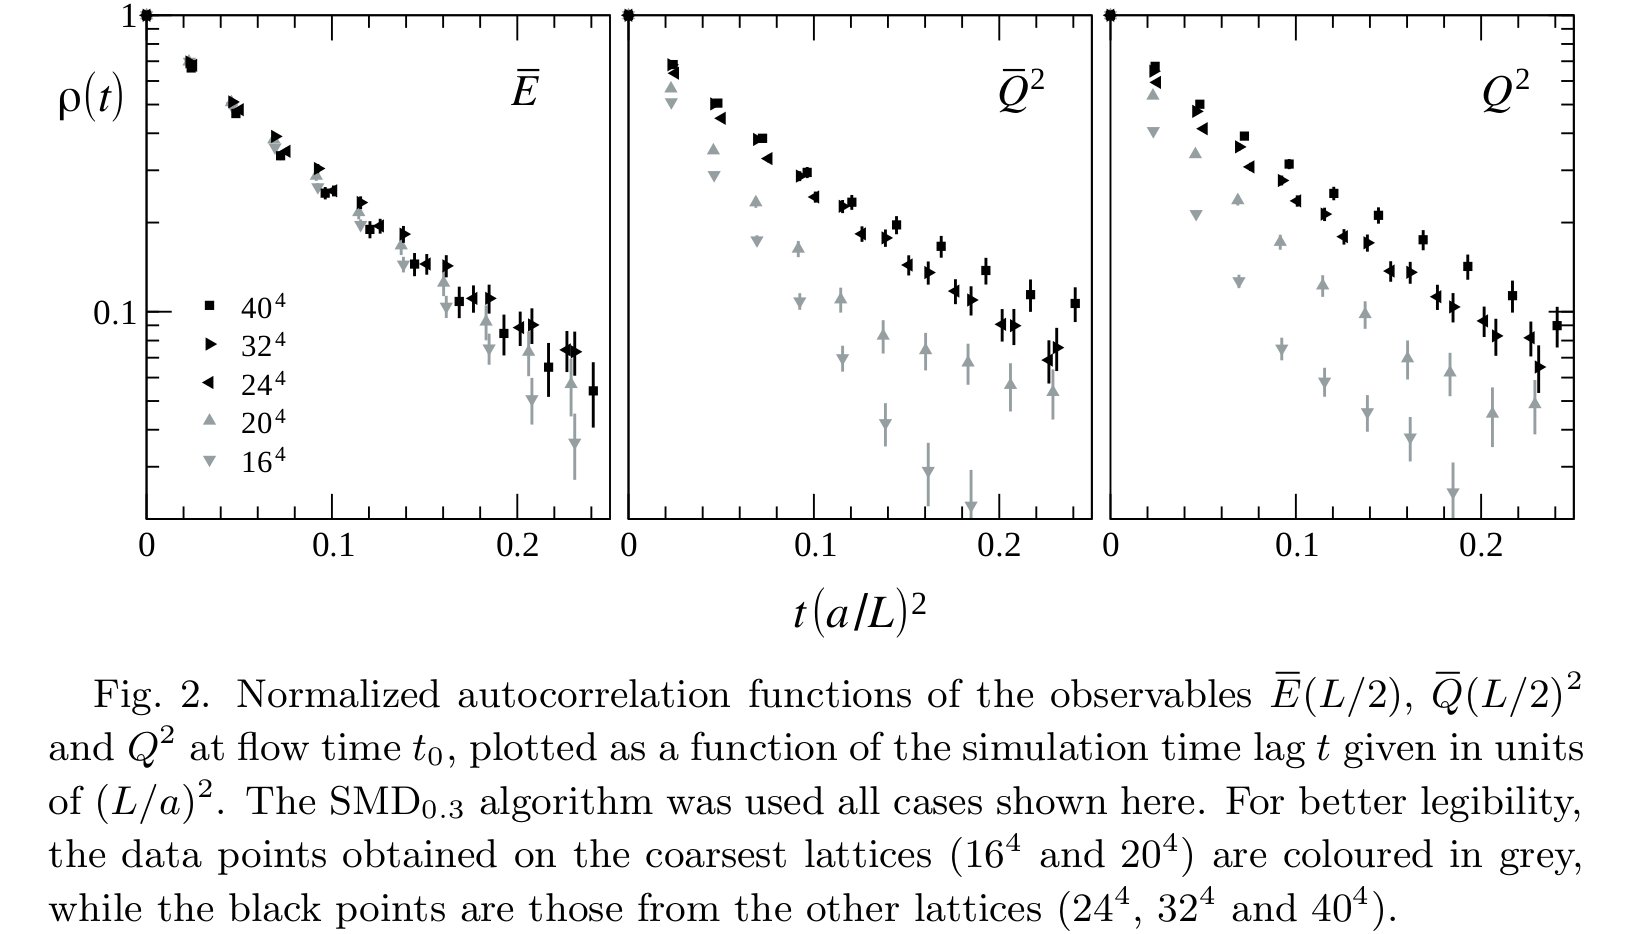
\includegraphics[width=0.8\textwidth]{autocorr.png}
    \end{figure}
\end{frame}

\begin{frame}{Some Real Data for Free-Theory}
    \begin{figure}
        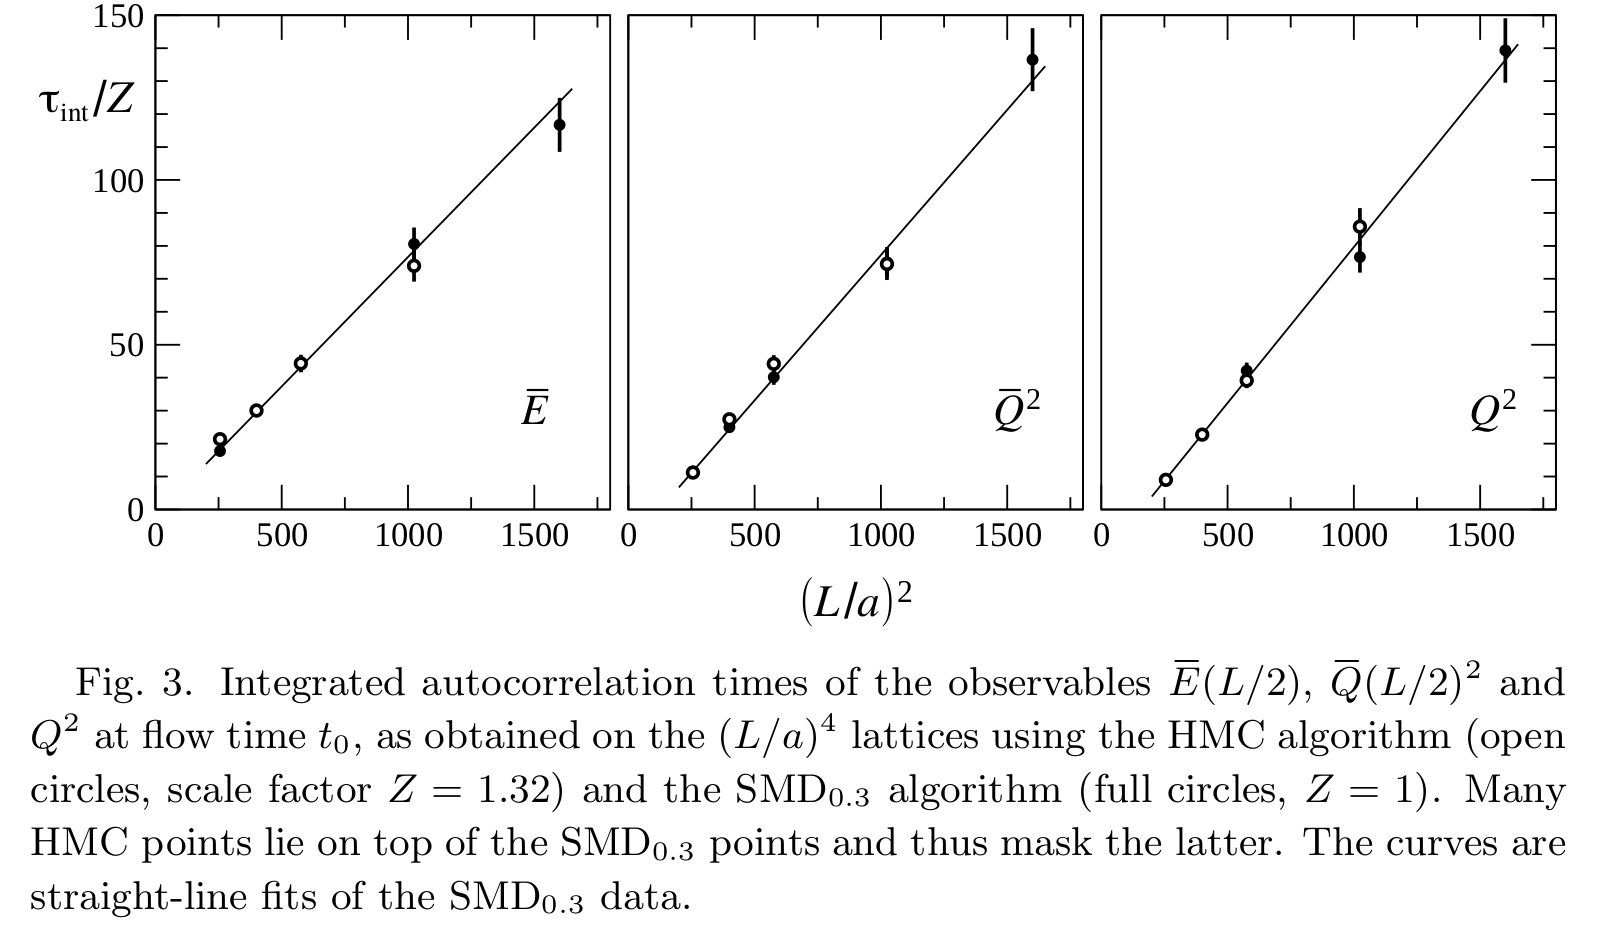
\includegraphics[width=0.8\textwidth]{scaling.png}
    \end{figure}
\end{frame}

\begin{frame}{A Small Test}
    Let's consider the harmonic oscillator in one dimension with action:
    \[
        S[x] = \sum_{i=1}^{N-1}\left[\frac{m}{2a}(x_i - x_{i+1})^2 + \frac{a}{2}\left(V(x_i) + V(x_{i+1})\right)\right]
    \]
    and try to sample the ground state energy defined as $E=\langle x^2\rangle$ using the Metropolis, the HMC and Langevin algorithms. 
\end{frame}

\begin{frame}{Metropolis Code}
    \begin{figure}
        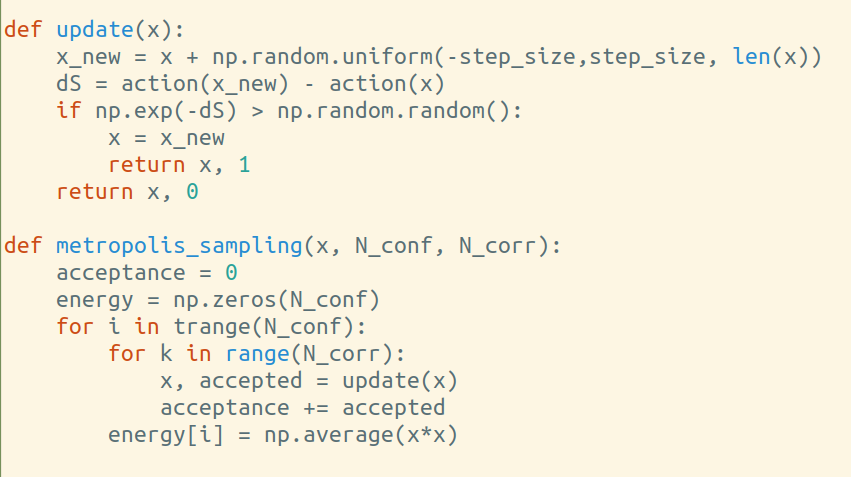
\includegraphics[width=0.8\textwidth]{metropolis_code.png}
    \end{figure}
\end{frame}

\begin{frame}{HMC Code}
    \begin{figure}
        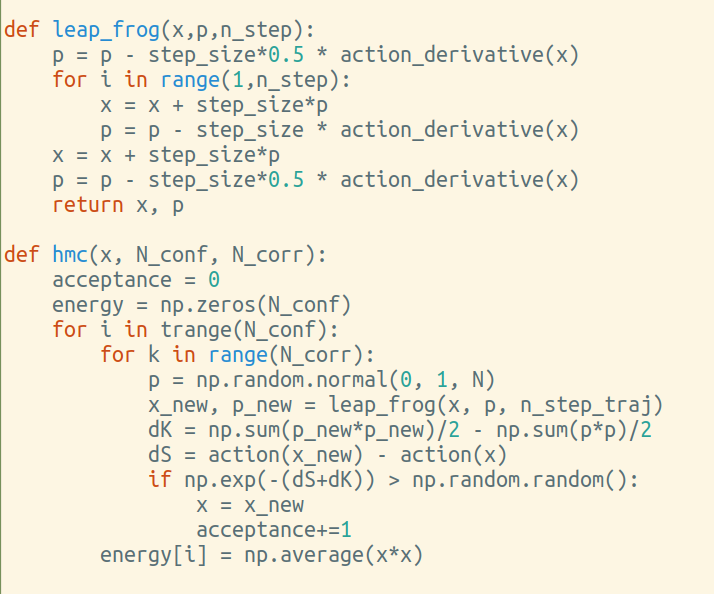
\includegraphics[width=0.8\textwidth]{hmc_code.png}
    \end{figure}
\end{frame}

\begin{frame}{Langevin Code}
    \begin{figure}
        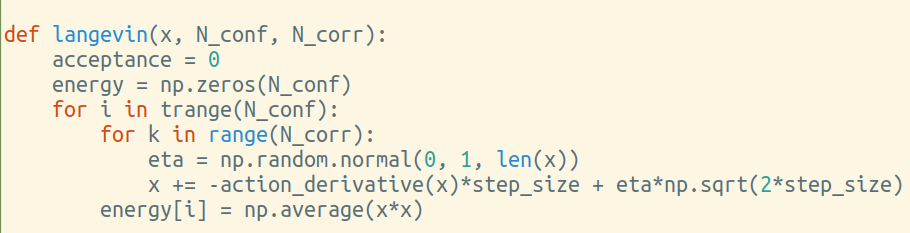
\includegraphics[width=0.8\textwidth]{langevin_code.png}
    \end{figure}
\end{frame}

\begin{frame}{Sample Monte Carlo Histories}
    \begin{figure}
        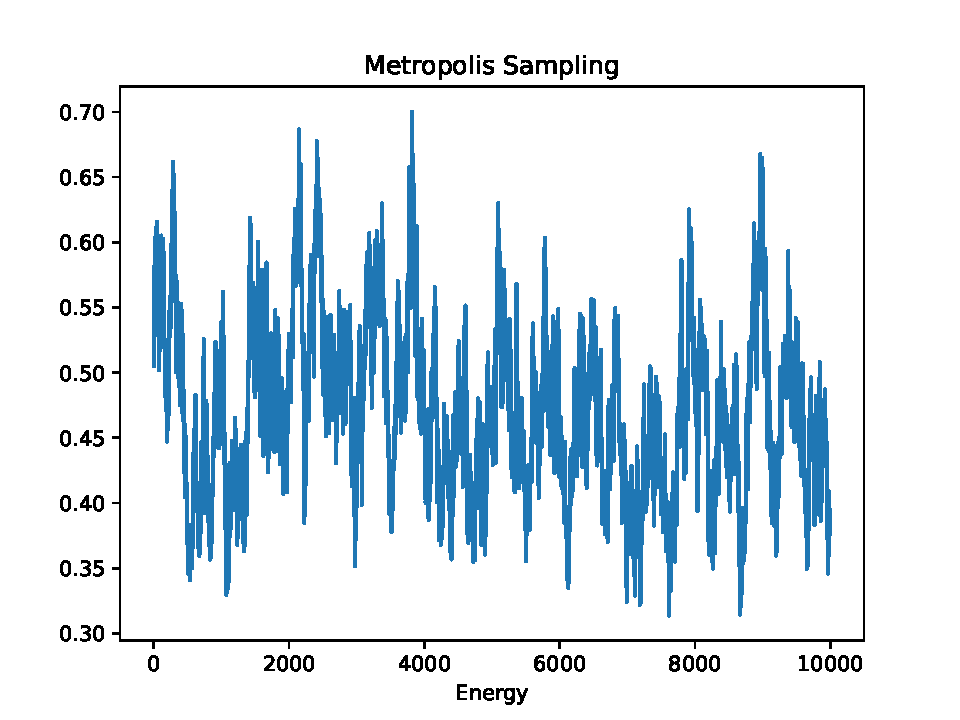
\includegraphics[width=0.5\textwidth]{metropolis.pdf}
        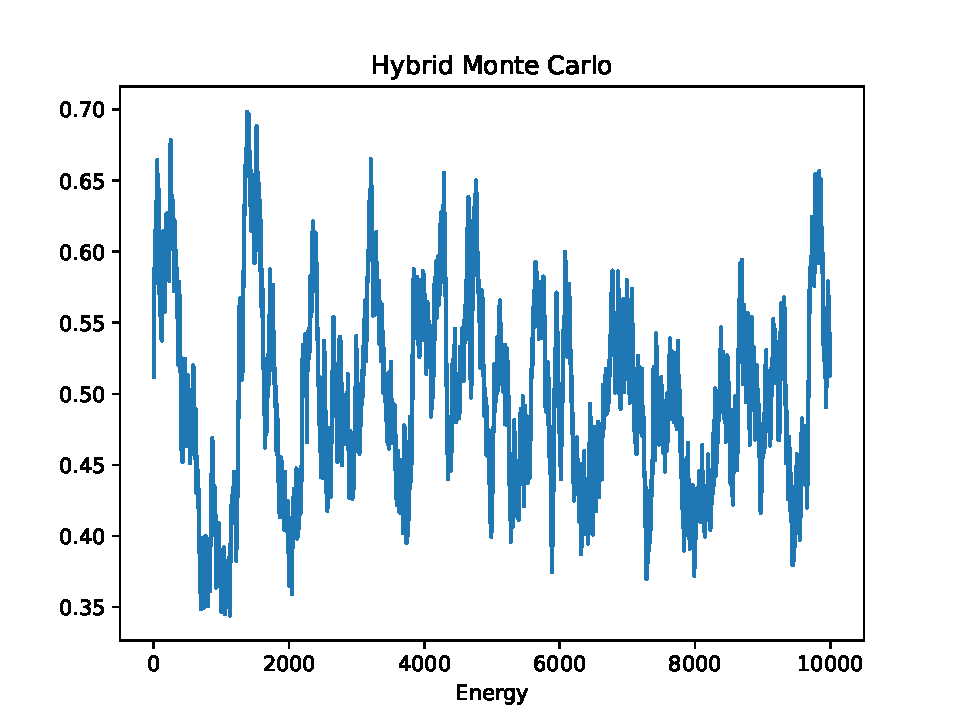
\includegraphics[width=0.5\textwidth]{hmc.pdf}
    \end{figure}
    \vspace{-0.5cm}
    \begin{figure}
        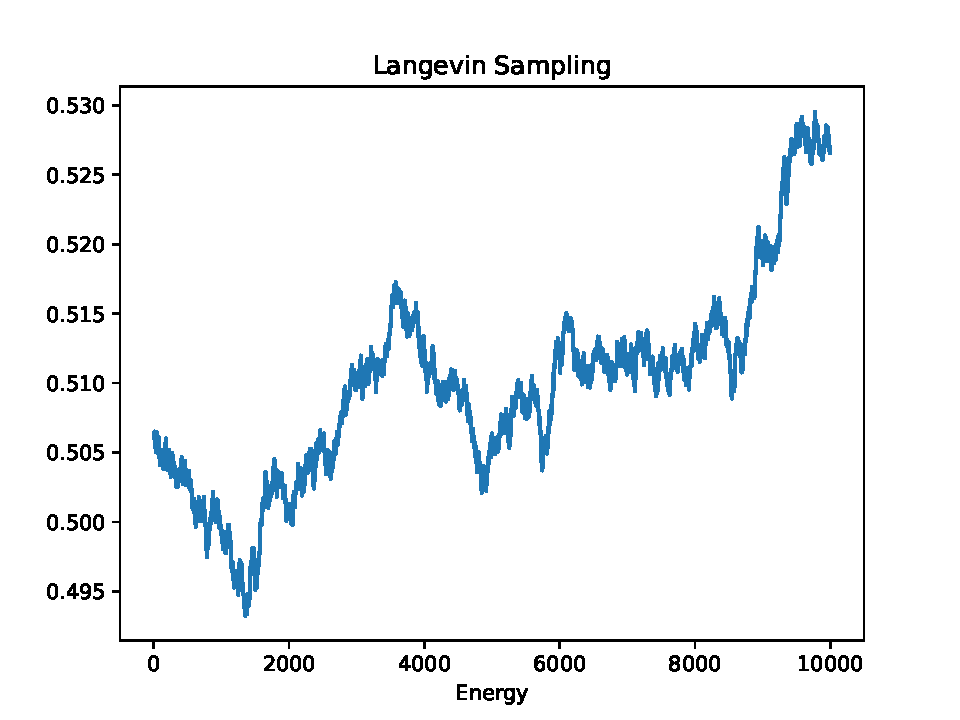
\includegraphics[width=0.5\textwidth]{langevin.pdf}
    \end{figure}
\end{frame}

\begin{frame}{Estimation of $\tau_{int}$}
The autocorrelation function is defined as:
    \[
    \Gamma(t) = \Gamma(-t) = \langle (x_i - \bar x)(x_{i+t} - \bar x)\rangle \approx \frac{1}{N-t}\sum_{i=1}^{N-t}  (x_i - \bar x)(x_{i+t} - \bar x),
\] 
where $t$ is the ``lag'' between two points. The integrated autocorrelation time is given by:
\[
    \tau_{int} = \frac{1}{2} \sum_{t=1}^\infty \frac{\Gamma(t)}{\Gamma(0)} = \frac{1}{2} \sum_{t=1}^\infty \rho(t).
    \label{autocorr:inf}
\]
In order to truncate the infinite summation one can look at the deviation squared of $\rho(t)$:
\[
    \langle \delta \rho(t)^2\rangle \approx \frac{1}{N} \sum_{k=1}^\infty \left[ \rho(k+t) + \rho(k-t) - 2\rho(k)\rho(t)\right]^2.
\]
All these terms, for a sufficiently large value of $k$ should all vanish, hence one can choose a cutoff $\Lambda$ and truncate the sum up to $t+\Lambda$. The integrated autocorrelation time, if the deviations of $\rho(t)$ become small, plateaus.
\end{frame}

\begin{frame}{Windowing Procedure for $\tau_{int}$ }
We choose a cutoff $W$ such that:
\[
    \tau_{int} = \frac{1}{2} \sum_{t=1}^W \rho(t),
    \label{autocorr_time}
\]
where $W$ is the first lag $t$ for which $\rho(t) < \sqrt{ (\langle \delta \rho(t)^2\rangle}$, when the contribution to the integration of $\tau_{int}$ from that lag become smaller than the deviation of that same lag. \\
An approximate error estimate of the integrated autocorrelation time can be defined as:
\[
    \sigma^2(\tau_{int}) \approx \frac{2(2W+1)}{N}\tau_{int}^2
    \label{eq:tauint_error}
\]
\end{frame}

\begin{frame}{Results}
    \centering
    \begin{figure}
        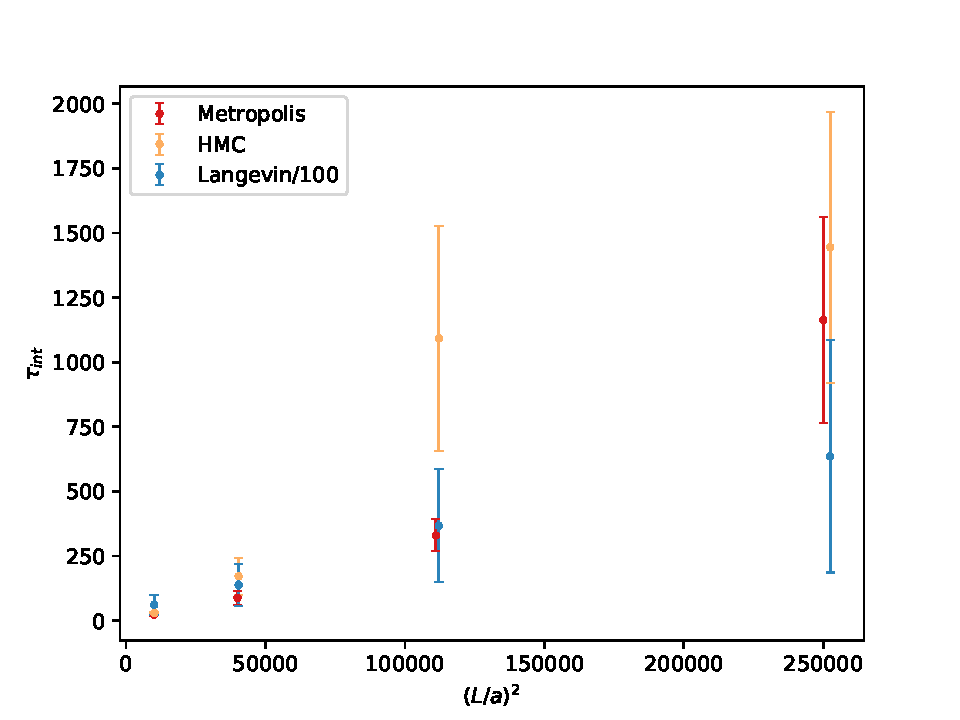
\includegraphics[width=0.8\textwidth]{tau_ints.pdf}
    \end{figure}
\end{frame}

\section{Conclusions}

\begin{frame}{Sources}
    
\begin{thebibliography}{99}
\bibitem{luscher_flow}
        M. L{\"{u}}scher , S. Schaefer,
        {\em Non-renormalizability of the HMC algorithm},
        (2011),
        Journal of High Energy Physics
\bibitem{luscher_flow_}
        M. L{\"{u}}scher , S. Schaefer,
        {\em Lattice QCD without topology barriers},
        (2011),
        Journal of High Energy Physics
\bibitem{zinn}
        J. Zinn-Justin,
        {\em Quantum Field Theory and Critical Phenomena},
        (1996),
\bibitem{gattringer}
        C.Gattringer, C.B. Lang,
        {\em Quantum Chromodynamics on the Lattice}
        (2010),
        Springer
\bibitem{sommer}
        R. M. Neal, 
        {\em MCMC using Hamiltonian dynamics},
        Chapter 5 of the "Handbook of Markov Chain Monte Carlo"
\end{thebibliography}
\end{frame}
\end{document}

